\documentclass{beamer}
\usetheme{Berlin}
\usepackage[OT1]{fontenc}
\usepackage{enumerate}
\usepackage[spanish]{babel}
\usepackage{enumitem}
\usepackage[utf8]{inputenc}
\usepackage{amsmath}
\usepackage{amsfonts}
\usepackage{amssymb}
\usepackage{amsthm}
\usepackage{graphicx}
\usepackage[labelformat=simple]{subcaption}
\usepackage{verbatim}
\usepackage{pgf}
\usepackage{tikz,braids}
\usepackage{listings}
\usepackage{leftidx}
\usepackage[all]{xy}
\usetikzlibrary{positioning}
\usepackage[export]{adjustbox}
\usepackage{csvsimple}
\usepackage{scrextend}
\begin{document}
\title{Grupo de trenzas y su aplicación en criptografía}   
\author{Fernando de la Hoz Moreno} 
\date{} 

\frame{\titlepage} 







\begin{frame}
\frametitle{Emil Artin} 

\begin{minipage}{.5\textwidth}

\begin{itemize}
\item Matemático austriaco (1898-1962).
\item Universidad de Gotinga y Universidad de Princeton.
\item Teoría de números, teoría algebraica de anillos asociativos y en los números hipercomplejos.
\item Acuñó los términos \textit{trenza} y \textit{grupo de trenzas} por primera vez en el año 1925.
\end{itemize}


\end{minipage}\hfill
\begin{minipage}{.5\textwidth}
\begin{figure}
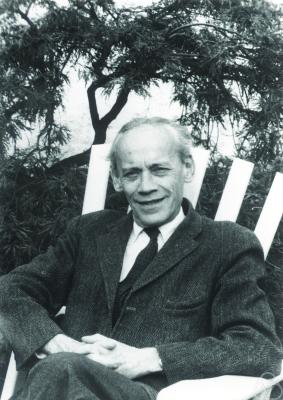
\includegraphics[height=0.9\textwidth]{imgs/EmilArtin}
\caption{Fotografía de Emil Artin.}
\end{figure}
\end{minipage}

\end{frame}







\begin{frame}
\frametitle{Trenza Geométrica}

Una \textbf{trenza geométrica} de $n$ hebras, con $n \geq 1$, es un subconjunto $\mathcal{B}\subset\mathbb{R}^2\times I$ formado por $n$ intervalos topológicos (subconjuntos de $\mathbb{R}^2\times I$ homeomorfos al intervalo $[0,1]$) disjuntos llamados hebras de tal manera que la proyección $\mathbb{R}^2\times I\rightarrow I$ establezca un homeomorfismo de cada hebra en $I$ y
$$\mathcal{B}\cap(\mathbb{R}^2\times \{0\})=\{(1,0,0),(2,0,0),...,(n,0,0)\},$$
$$\mathcal{B}\cap(\mathbb{R}^2\times \{1\})=\{(1,0,1),(2,0,1),...,(n,0,1)\}.$$
Cada hebra de $\mathcal{B}$ interseca con el plano $\mathbb{R}^2\times \{t\}$ con $t\in I$ en un único punto y conecta un punto $(i,0,0)$ con un punto $(s(i),0,1)$ donde $i,s(i)\in\{1,2,...,n\}$. La sucesión $(s(1),s(2),...,s(n))$ es una permutación del conjunto $\{1,2,...,n\}$ llamada permutación subyacente de $\mathcal{B}$.
\end{frame}





\begin{frame}
\frametitle{Trenza Geométrica}

\begin{figure}
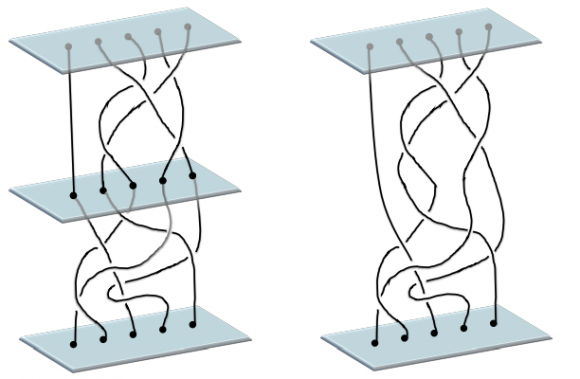
\includegraphics[height=0.5\textwidth]{imgs/trenza_geo}
\caption{Trenza Geométrica.}
\end{figure}

\end{frame}


\begin{frame}
\frametitle{Isotopía}


Dos trenzas geométricas $\mathcal{B}$ y $\mathcal{B}'$ son \textbf{isotópicas} si podemos deformar de manera continua $\mathcal{B}$ en $\mathcal{B}'$.
\newline

La relación de isotopía establece una relación de equivalencia y al conjunto de clases de equivalencia se les denomina \textbf{trenzas de n hebras}, denotándolo por $\mathcal{B}_n$.


\end{frame}


\begin{frame}
\frametitle{Diagrama de trenzas}

\begin{figure}
\centering

\begin{tikzpicture}
\braid[line width =1.5pt, number of strands = 5, name = b1, height = 25pt] (b1) at (-7,0)  a_1^{-1} a_4 a1 a_2 a_3;

\end{tikzpicture}

\end{figure}

\end{frame}





\begin{frame}
\frametitle{Producto de trenzas}

Sean $\beta_1,\beta_2\in \mathcal{B}_3$, cuyos diagramas se pueden ver en (a), el resultado del producto $\beta_1\beta_2$ se representa en (b).
\begin{figure}
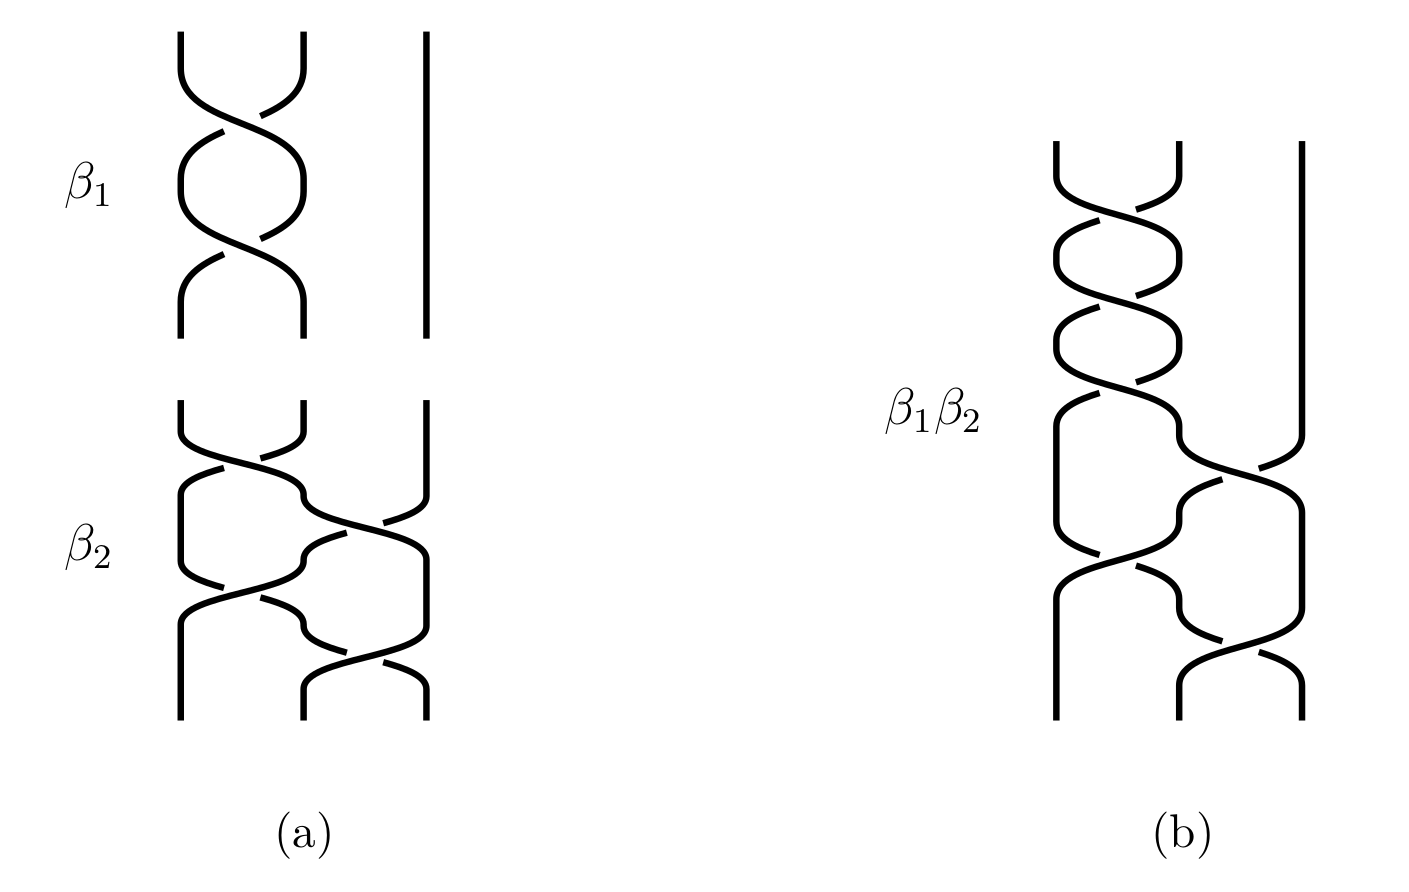
\includegraphics[scale=0.15]{imgs/imgs_trenzas/producto}
\end{figure}

\end{frame}


\begin{frame}
\frametitle{Asociatividad}


\begin{figure}
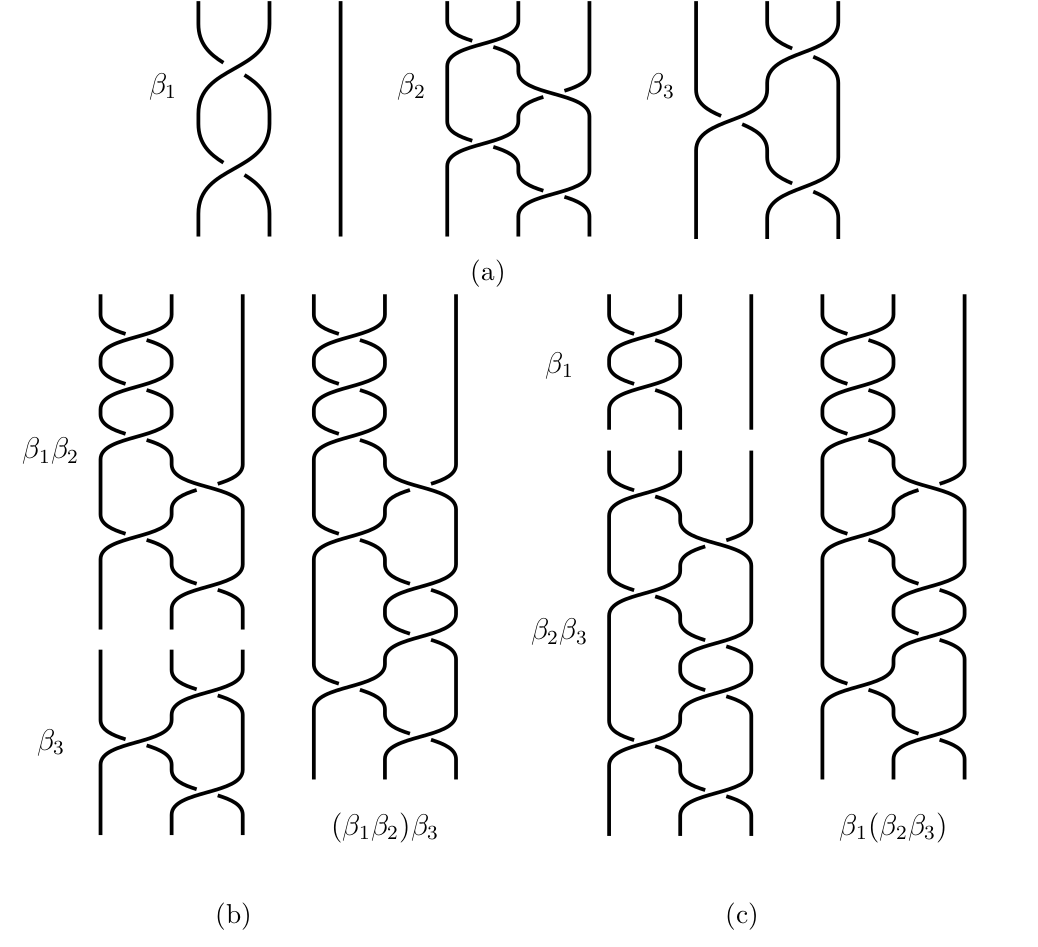
\includegraphics[scale=0.198]{imgs/imgs_trenzas/asociatividad}
\end{figure}

\end{frame}


\begin{frame}
\frametitle{Elemento neutro}

\begin{figure}[h!]
\begin{center}
		\begin{tikzpicture}
		\braid[line width =1.5pt, height = 50pt, number of strands = 2, name = a]  a1;
		\node[at=(a-1-s),pin=north west:1]  {};
		\node[at=(a-2-s),pin=north west:2]  {};
		\node[] at (3,-1){$\cdot\cdot\cdot$};
		\braid[line width =1.5pt, height = 50pt, number of strands = 2, name = b] at (4,0) a1;
		\node[at=(b-1-s),pin=north west:$n-1$]  {};
		\node[at=(b-2-s),pin=north west:$n$]  {};
		\end{tikzpicture}
		\end{center}

\end{figure}


\end{frame}

\begin{frame}
\frametitle{Trenzas elementales}


\begin{figure}
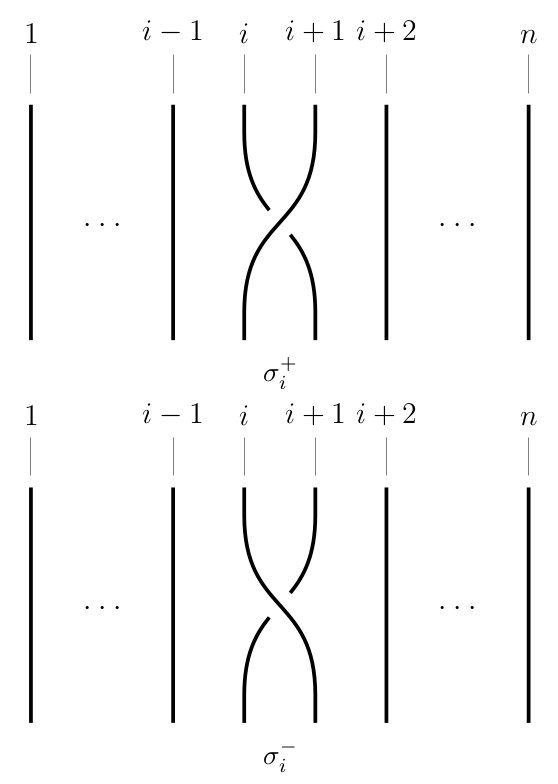
\includegraphics[scale=0.23]{imgs/imgs_trenzas/trenzas_elementales}
\end{figure}

\end{frame}

\begin{frame}
\frametitle{Inverso}

\begin{block}{Lema}
El conjunto de trenzas elementales genera $\mathcal{B}_n$ como monoide.
\end{block}

\begin{block}{Colorario}
Sea $\beta\in\mathcal{B}_n$, existe un elemento $\beta^{-1}\in\mathcal{B}_n$ que es el inverso por ambos lados de $\beta$.
\end{block}

\begin{exampleblock}{Ejemplo}
$$\beta = \sigma_3^+\sigma_1^-\sigma_5^+\sigma_2^+\ \ \ \ \ \beta^{-1}=\sigma_2^-\sigma_5^-\sigma_1^+\sigma_3^-$$
\end{exampleblock}

\end{frame}


\begin{frame}
\frametitle{Grupo de trenzas de Artin}

El \textbf{grupo de trenzas de Artin} $B_n$ es el grupo generado por $n-1$ elementos $\sigma_1, \sigma_2,...,\sigma_{n-1}$ y las relaciones de trenza
$$\sigma_i\sigma_j = \sigma_j\sigma_i,$$
para todo $i,j\in\{1,2,...,n-1\}$ con $|i-j|\geq 2$ y

$$\sigma_i\sigma_{i+1}\sigma_i =\sigma_{i+1}\sigma_i\sigma_{i+1},$$
para todo $i\in\{1,2,...,n-2\}$.

\end{frame}

\begin{frame}
\frametitle{Grupo de trenzas de Artin}

\begin{block}{Teorema}
Para $\varepsilon \in\{+,-\}$, existe un único homomorfismo $\varphi_\varepsilon : B_n\rightarrow\mathcal{B}_n$ tal que $\varphi_\varepsilon(\sigma_i) = \sigma_i^\varepsilon$ para cada $i\in\{1,2,...,n-1\}$. El homomorfismo $\varphi_\varepsilon$ es un \textbf{isomorfismo}.
\end{block}
\end{frame}


\begin{frame}
\frametitle{Plataformas criptográficas}

Una \textbf{plataforma criptográfica} es un método criptográfico basado en un  objeto matemático. Si este objeto es un grupo, se le denomina \textbf{grupo plataforma}. La seguridad de la plataforma depende de la dificultad, computacional o teórica, de resolver un problema de teoría de grupos en el grupo plataforma.
\end{frame}

\begin{frame}
\frametitle{Plataformas criptográficas}

Entre las propiedades que necesita un grupo de plataforma se encuentran:
\begin{itemize}
\item Una \textbf{representación finita}.
\item Una \textbf{forma normal} para representar de forma única a los elementos del grupo.
\item Un \textbf{problema $\mathcal{P}$} de teoría de grupos que sea generalmente complejo.
\end{itemize}
\end{frame}

\begin{frame}
\frametitle{Problema del conjugado}
\begin{block}{Definición}
El \textbf{problema del conjugado} en el grupo $B_n$ consiste en encontrar un procedimiento que nos permita, dados $\alpha,\beta\in B_n$, decidir si existe $\gamma\in B_n$ tal que $\alpha=\gamma\beta\gamma^{-1}$.
\end{block}
\end{frame}



\begin{frame}
\frametitle{Monoide de Garside}
Un \textbf{monoide de Garside exhaustivo} es un par $(M,\Delta)$, donde $M$ es un monoide y $\Delta$ un elemento de $M$ (\textbf{elemento de Garside}) que cumplen ciertas características. Consideramos $G_M$ como el grupo de fracciones de $M$. Algunas de las propiedades que nos proporciona un monoide de Garside exhaustivo son:
\begin{itemize}
\item Obtenemos una \textbf{forma normal} en $G_M$.
\item Da una \textbf{solución} al problema del conjugado en $G_M$.
\end{itemize}

\end{frame}

\begin{frame}
\frametitle{Monoide de Garside}
Para cualquier $n\geq 1$, denotamos por $B_n^+$ el monoide generado por $n-1$ generadores $\sigma_1,\sigma_2,\ldots,\sigma_{n-1}$ y las relaciones
$$\sigma_i\sigma_j=\sigma_j\sigma_i\ \ \ si\ |i-j|\geq 2,$$
$$\sigma_i\sigma_j\sigma_i=\sigma_j\sigma_i\sigma_i\ \ \ si\ |i-j|= 1,$$
donde $i,j\in\{1,2,\ldots,n-1\}$. El monoide $B_n^+$ se llama \textbf{monoide de trenzas} de $n$ hebras. Consideramos el elemento de Garside $$\Delta_n =(\sigma_1\cdots\sigma_{n-2}\sigma_{n-1})(\sigma_1\cdots\sigma_{n-2})\cdots(\sigma_1\sigma_2)\sigma_1$$
Entonces $(B_n^+,\Delta_n)$ es un monoide de Garside exhaustivo y $G_{B_n^+}=B_n$.
\end{frame}

\begin{frame}
\frametitle{Anshel-Anshel-Goldfeld}

Es un método de intercambio de llave público propuesto por Anshel \& al en 1999. 
La llave pública consiste en dos conjuntos de trenzas $\{p_1,...,p_l\},\{q_1,...,q_m\}\subset B_n$. La llave secreta es una palabra formada a partir de estos conjuntos.
\newline

La seguridad está basada en la dificultad de resolver una variante del Problema de Búsqueda del Conjugado en $B_n$, que es llamado el Problema de Búsqueda del conjugado Múltiple, en el cual se intenta encontrar una trenza conjugadora  de una familia finita de pares de trenzas $(p_1,p_1'),...,(p_l,p_l')$.

\end{frame}

\begin{frame}
\frametitle{Anshel-Anshel-Goldfeld}

\begin{figure}
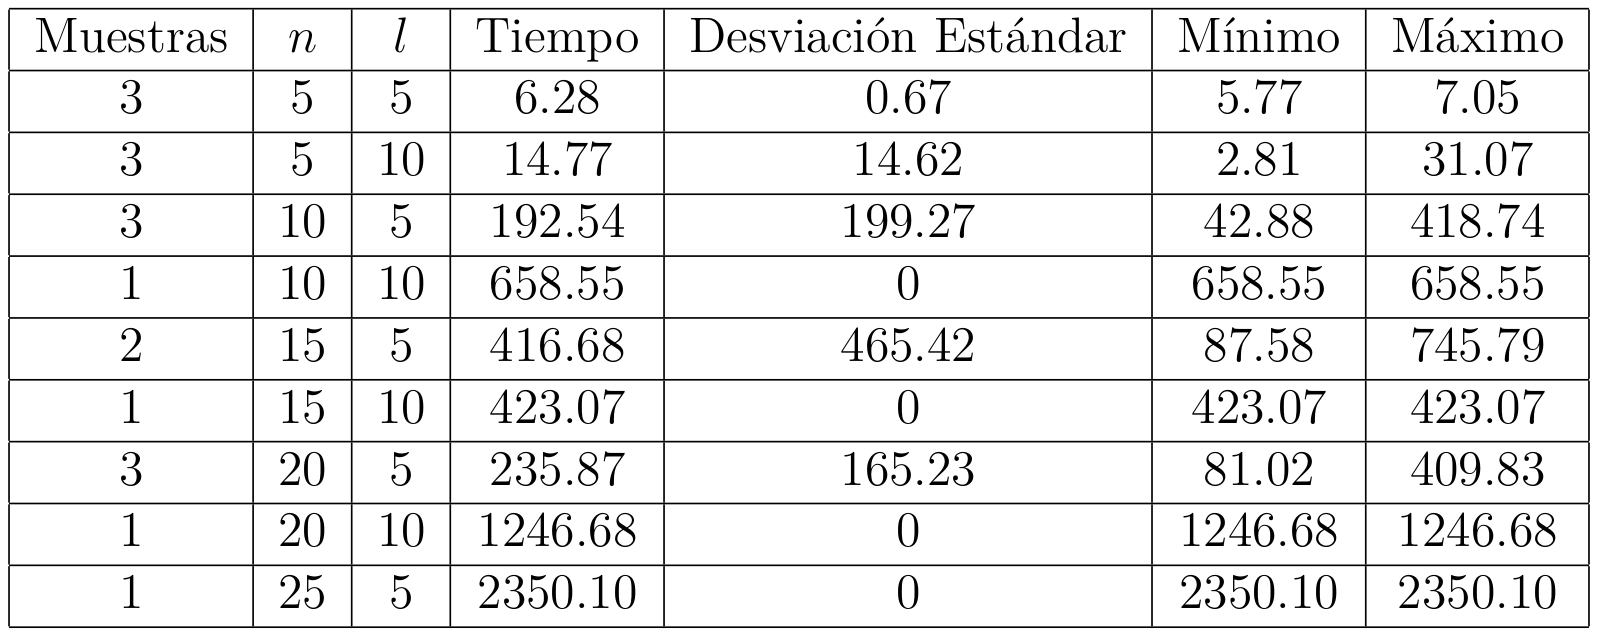
\includegraphics[scale=0.198]{imgs/imgs_trenzas/result_anshel}
\end{figure}

\end{frame}


\begin{frame}
\frametitle{Diffie-Helman}

Este esquema de intercambio de llave Diffie-Hellman es propuesto por Ko, Lee \& al. En él hace uso de subgrupos de $B_n$, donde los elementos de uno conmutan con los elementos de otro. En concreto se utilizan los subgrupos $LB_n =\langle\sigma_1,...,\sigma_{m-1}\rangle$ y  $UB_n=\langle\sigma_{m+1},...,\sigma_{n-1}\rangle$ con $m=[n/2]$. La llave pública es una trenza de $B_n$ y las llaves privadas son trenzas de $LB_n$ y $UB_n$.
\newline

La seguridad también está basada en la dificultad de resolver una variante del Problema de Búsqueda del Conjugado donde dada una trenza $p$ de $B_n$ y las trenzas $p'=sps^{-1}$ y $p''=rpr^{-1}$, con $s$ y $r$ pertenecientes a $LB_n$ y $UB_n$ respectivamente, hay que encontrar la trenza $rp'r^{-1}$ o $sp''s^{-1}$.

\end{frame}


\begin{frame}
\frametitle{Diffie-Helman}

\begin{figure}
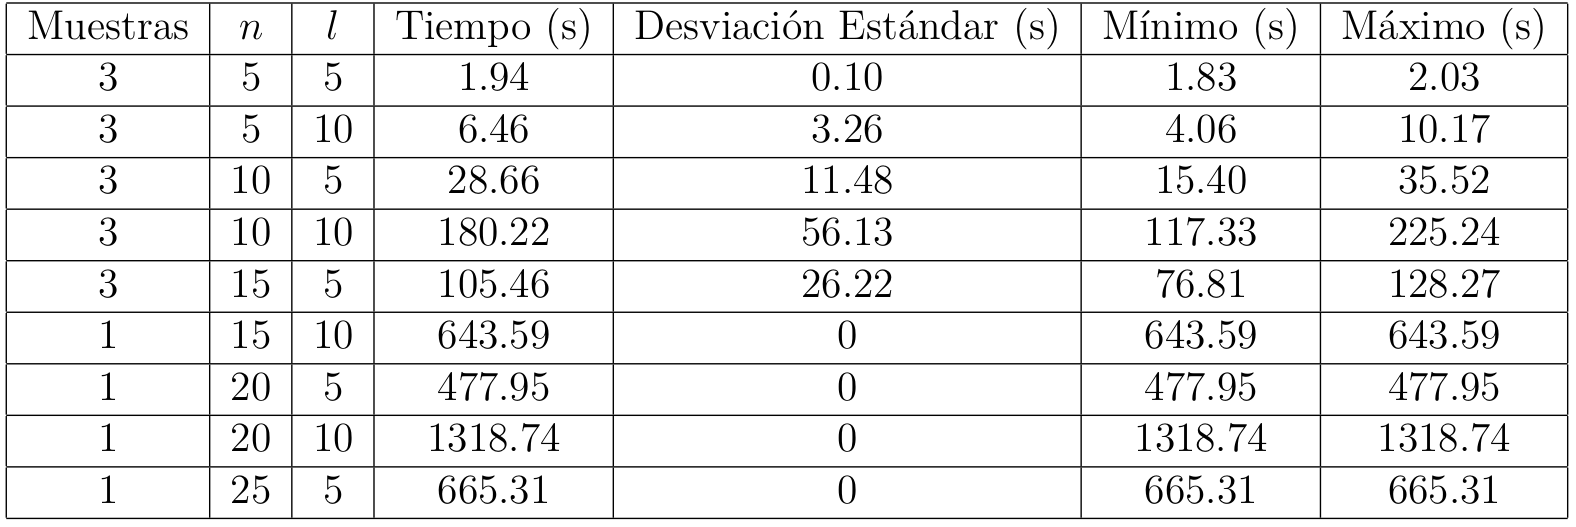
\includegraphics[scale=0.198]{imgs/imgs_trenzas/result_ko}
\end{figure}

\end{frame}



\begin{frame}
\frametitle{Criptoanálisis}
Ataques al problema de la búsqueda del conjugado:
\begin{itemize}
\item Super conjuntos cumbre.
\item Ataques basados en longitud.
\item Ataques teóricos de representación.
\end{itemize}


\end{frame}


\begin{frame}
\frametitle{Heurística}

\begin{figure}
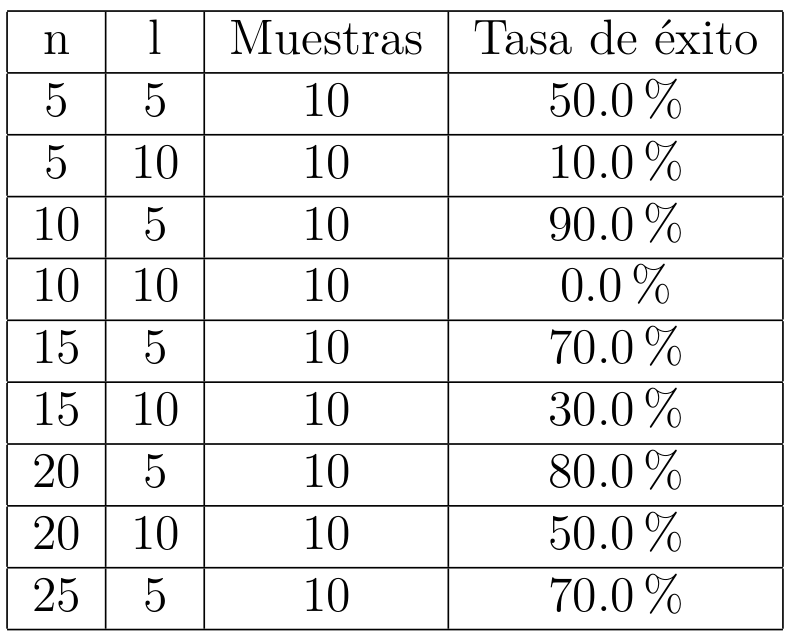
\includegraphics[scale=0.198]{imgs/imgs_trenzas/result_heur}
\end{figure}

\end{frame}


\begin{frame}
\frametitle{Bibliografía}

\begin{thebibliography}{X}
\bibitem{Art1}\textsc{Emil Artin}, \textit{Theorie der z\"opfe}, 1925.
\bibitem{Art2}\textsc{Emil Artin}, \textit{Theory of braids}, Vol. 48, No. 1, January, 1947.
\bibitem{Deh}\textsc{Patrick Dehornoy}, \textit{Braid-based cryptography}.
\bibitem{Alg}\textsc{Elsayed A. Elrifai},\textsc{Hugh R. Morton}, \textit{Algorithms for positive braids}.
\bibitem{Att}\textsc{Dennis Hofheinz},\textsc{Rainer Steinwandt}, \textit{A Practical Attack on Some Braid Group Based
Cryptographic Primitives}.
\bibitem{group}\textsc{Stevev Roman}, \textit{Fundamentals of group theory. An advance aproach}.
\bibitem{wiki}\textit{Algebra abstracta}\newline https://es.wikibooks.org/wiki/Matemáticas\_Universitarias/Álgebra\_Abstracta
\bibitem{alg_abs}\textsc{Pierre Antoine Brillet}, \textit{Abstract algebra}. 2007.
\bibitem{free}\textsc{B. Suri}, \textit{Free groups - basics}. 2010.
\bibitem{monoides}\textsc{John M. Howie}, \textit{Fundamentals of semigroup theory}.
\bibitem{br_gr}\textsc{Christian Kassel}, \textsc{Vladimir Turaev}, \textit{Braid groups}.
\bibitem{st_br}\textsc{Kunio Murasugi}, \textsc{Bohdan l. Kurpita}, \textit{A study of braids}.
\bibitem{in_cr}\textsc{Hans Delfs}, \textsc{Helmut Knebl}, \textit{Introduction to cryptography. Principles and Applications.}

\bibitem{co_ma}\textsc{Gilbert Baumslag}, \textsc{Benjamin Fine},  \textsc{Martin Kreuzer}, \textsc{Gerhard Rosenberger},\textit{A course in mathematical cryptography.}

\bibitem{AAG}\textsc{I. Anshel}, \textsc{M. Anshel}, \textsc{D. Goldfeld}, \textit{New key agreement protocols in braid group cryptography}. 2001.


\bibitem{Ko}\textsc{K.H. Ko}, \textsc{S.J. Lee}, \textsc{J.H. Cheon}, \textsc{J.W. Hang}, \textsc{J.S. Kang}, \textsc{C. Park}, \textit{New public-key cryptosystem using braid groups}. 2000.

\bibitem{Ko_sig}\textsc{K.H. Ko}, \textsc{P. Dehornoy}, \textsc{M. Girault}, \textsc{J.W. Lee}, \textit{New signature scheme using conjugacy problem, Preprint}. 2002.

\bibitem{Sibert}\textsc{H. Sibert}, \textsc{D.H. Choi}, \textsc{M.S. Cho}, \textsc{J.W. Lee}, \textit{Entity authentication schemes using braid word reduction}. 2003.

\bibitem{Emil}\textit{Imagen de Emil Artin}. De Konrad Jacobs, Erlangen - Mathematisches Forschungsinstitut Oberwolfach, https://opc.mfo.de/detail?photoID=116, CC BY-SA 2.0 de, https://commons.wikimedia.org/w/index.php?curid=3898471


\bibitem{sa_br}\textit{Manual Sage. Grupo de trenzas.}\newline https://doc.sagemath.org/html/en/reference/groups/sage/groups/braid.html
\bibitem{sa_pe} \textit{Manual Sage. Grupo de permutaciones.}\newline https://doc.sagemath.org/html/en/reference/groups/sage/groups/perm\_gps/\newline permgroup\_element.html
\end{thebibliography}




\end{frame}



\begin{frame}
\frametitle{Bibliografía}

\begin{thebibliography}{X}

\bibitem{alg_abs}\textsc{Pierre Antoine Brillet}, \textit{Abstract algebra}. 2007.
\bibitem{free}\textsc{B. Suri}, \textit{Free groups - basics}. 2010.
\bibitem{monoides}\textsc{John M. Howie}, \textit{Fundamentals of semigroup theory}.
\bibitem{br_gr}\textsc{Christian Kassel}, \textsc{Vladimir Turaev}, \textit{Braid groups}.
\bibitem{st_br}\textsc{Kunio Murasugi}, \textsc{Bohdan l. Kurpita}, \textit{A study of braids}.
\bibitem{in_cr}\textsc{Hans Delfs}, \textsc{Helmut Knebl}, \textit{Introduction to cryptography. Principles and Applications.}

\bibitem{co_ma}\textsc{Gilbert Baumslag}, \textsc{Benjamin Fine},  \textsc{Martin Kreuzer}, \textsc{Gerhard Rosenberger}, \textit{A course in mathematical cryptography.}


\end{thebibliography}




\end{frame}




\begin{frame}
\frametitle{Bibliografía}

\begin{thebibliography}{X}


\bibitem{AAG}\textsc{I. Anshel}, \textsc{M. Anshel}, \textsc{D. Goldfeld}, \textit{New key agreement protocols in braid group cryptography}. 2001.


\bibitem{Ko}\textsc{K.H. Ko}, \textsc{S.J. Lee}, \textsc{J.H. Cheon}, \textsc{J.W. Hang}, \textsc{J.S. Kang}, \textsc{C. Park}, \textit{New public-key cryptosystem using braid groups}. 2000.

\bibitem{Ko_sig}\textsc{K.H. Ko}, \textsc{P. Dehornoy}, \textsc{M. Girault}, \textsc{J.W. Lee}, \textit{New signature scheme using conjugacy problem, Preprint}. 2002.

\bibitem{Sibert}\textsc{H. Sibert}, \textsc{D.H. Choi}, \textsc{M.S. Cho}, \textsc{J.W. Lee}, \textit{Entity authentication schemes using braid word reduction}. 2003.

\bibitem{Emil}\textit{Imagen de Emil Artin}. De Konrad Jacobs, Erlangen - Mathematisches Forschungsinstitut Oberwolfach, https://commons.wikimedia.org/w/index.php?curid=3898471


\end{thebibliography}




\end{frame}


\end{document}